\section{Sample section}
\citeN{Laidlaw2001} compared the effectiveness of
visualization techniques by presenting test subjects with the task of
estimating where a particle placed in the center of a flow field
would exit a circle. Six different flow-field visualization methods
were assessed by comparing the difference between the actual exit
numerically calculated and the estimation of the exit by the human
subjects. Laidlaw et~al.'s experiment was carried out on humans but,
in our work, we apply this evaluation technique to humans as well as
to our model of the human visual system and use a streamline tracing
algorithm to trace the path of the particle.

We use the term streamline tracing to describe the higher level
process that must exist for people to judge a streamline pathway.
We call it streamline tracing because the task seems to require the
user to make a series of judgments, starting at the center, whereby
the path of a particle dropped in the center is integrated in a
stepwise pattern to the edge of the field. Though many algorithms
exist in the machine vision literature for contour tracing, we found
these to be inappropriate for use in this application. Contour
tracing algorithms are generally designed to trace out the boundary
of some shape but a streamline tracing algorithm must also be able
able to produce a streamline in a field of disconnected contours,
such as is the case with the regular arrows. The streamline to be
traced will often not follow a visible contour but instead be locate
between contours, and will sometimes pass through areas devoid of
visual elements. Thus we developed a specialized algorithm that is
capable of tracing streamlines that do not necessarily correspond to
the boundary of any shape but can pass between visual contours.

Perception is a combination of top-down and bottom-up processes.
Bottom-up processes are driven by information on the retina and are
what is simulated by Li's model \citeyear{Li1998a}. Top-down
processes are much more varied and are driven in the brain by
activation from regions in the frontal and temporal cortex that are
known to be involved in the control of pattern identification and
attention \cite{Lund2001}. All of the flow visualizations evaluated
by \citeN{Laidlaw2001}, except for LIC, contain symbolic information
regarding the direction of flow along the contour elements (e.g. an
arrowhead). In a perpetual/cognitive process this would be regarded
as a top-down influence. At present our model does not deal with
symbolic direction information but it does do streamline tracing once
set in the right general direction.

Streamline tracing is a combination of top-down and bottom-up
processes. Broadly speaking, top-down processes reflect task demands
and the bottom-up processes reflect environmental information. In our
case, the bottom-up information comes from the different types of
visualization, while the top-down information is an attempt to model
the cognitive process of streamline pathway tracing. Contour
integration was modeled using the following iterative algorithm.

% Algorithm
\medskip
\begin{algorithm}[H]
\SetAlgoNoLine
$current\_position \leftarrow$ center \\
$current\_direction \leftarrow$ up \\
$current\_position$ is inside circle \\
\While{$current\_position$ is inside circle,}{
  $neighborhood \leftarrow$ all grid hexes within two hexes from $current\_position$ \\
  \For{ each $hex$ in $neighborhood$, }{
  \For{each $neuron$ in $hex$}{
  convert $neuron\_orientation$ to $vector$ \\
  scale $vector$ by $neuron\_excitation$ \\
  $vector\_sum \leftarrow vector\_sum + vector$}}

  normalize $vector\_sum$ \\
  $current\_position \leftarrow current\_position + vector\_sum$ \\
  $current\_direction \leftarrow vector\_sum$ \\
return $current\_position$ \\
}
    \caption{Iterative Algorithm}
    \label{alg:one}
  \end{algorithm}
\medskip

The algorithm maintains a context that contains a current position
and direction. Initially, the position is the center, and the
direction set to upward. This context models the higher-order,
top-down influence on the algorithm that results from the task
requirements (tracing from the center dot) and the directionality
which in our experiment was set to be always in an upwardly trending direction.

The algorithm traces the contour by repeatedly estimating the flow
direction at the $current\_position$ and moving the position a small
distance (.5 hex radii) in that direction. The flow direction is
calculated from the neural responses in the local neighborhood of the
$current\_position$. The excitation of each neuron is used to
generate a vector whose length is proportional to the strength of the
response and whose orientation is given by the receptive field
orientation. Because receptive field orientations are ambiguous as to
direction (for any vector aligned with the receptive field, its
negative is similarly aligned). The algorithm chose the vector most
closely corresponding to the vector computed on the previous
iteration. Vectors are computed for all neurons in hypercolumns
within a 2-hexes radius of the current position; they are summed and
normalized to generate the next $current\_direction$.

Some changes were made from the method published by
\citeN{Pineo2008}. Previously, the algorithm considered only a single
hex cell at each iteration of the algorithm. We found that this would
occasionally cause unrealistically large errors in streamline
tracing. For example, on visualizations with arrowheads, the neural
network might yield a very strong edge orthogonal to the flow field
positioned at the back of an arrowhead. If the algorithm considered
only the edges at this point, it may make a significant error,
despite the edges in nearby positions indicating the correct
direction. We felt that creating an average over $neighborhood$ was
the more correct approach, and we found closer agreement with human
performance with this change.

\subsection{Qualitative Evaluation}
Four different flow visualization methods were used in our evaluation
of the theory. These were implementations of four of the six used by
\citeN{Laidlaw2001}. We chose to investigate a regular arrow grid
because it is still the most commonly used in practice and a jittered
arrow grid because of the arguments that have been made that this
should improve perceptual aliasing problems \cite{Turk1996}. We added
Line Integral Convolution (LIC) because of its widespread advocation
by the visualization community \cite{Cabral1993} and head-to-tail
aligned streaklets because of Laidlaw et al.'s finding that is was
the best and the theoretical arguments in support of this method
\cite{Ware2008}. Note that Laidlaw et al. used Turk and Banks
algorithm to achieve aligned arrows on equally spaced streamlines
while we used Jobard and Lefer's \citeyear{Jobard1997} method to
achieve the same effect and we used streaklets without an arrowhead
\cite{Fowler1989}.

\begin{figure}[tp]
    \begin{minipage}[t]{0.45\linewidth}
        \centering
        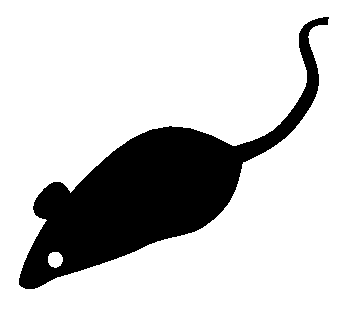
\includegraphics{./fig/acmlarge-mouse}
        \caption{Regular arrows.}
        \label{regularfig}
    \end{minipage}
    \hspace{0.1\linewidth}
    \begin{minipage}[t]{0.45\linewidth}
        \centering
        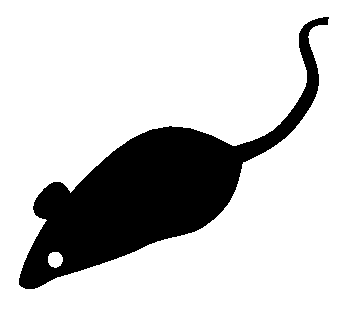
\includegraphics{./fig/acmlarge-mouse}
        \caption{Jittered arrows.}
        \label{jitteredfig}
    \end{minipage}
\end{figure}

\begin{figure}[tp]
    \begin{minipage}[t]{0.45\linewidth}
        \centering
        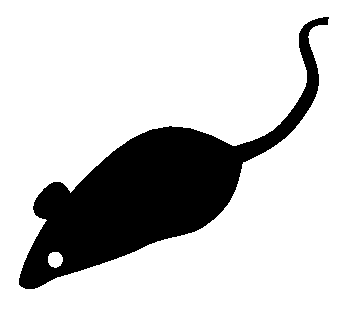
\includegraphics{./fig/acmlarge-mouse}
        \caption{Closeup of neural response to arrowheads.}
        \label{ortharrowheadfig}
    \end{minipage}
    \hspace{0.1\linewidth}
    \begin{minipage}[t]{0.45\linewidth}
        \centering
        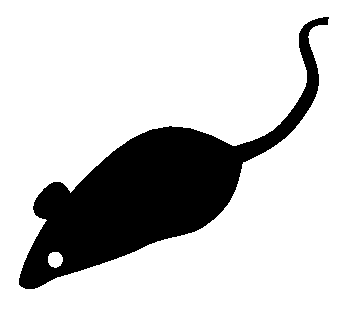
\includegraphics{./fig/acmlarge-mouse}
        \caption{Closeup of neural response to aligned streaklets.}
        \label{alignedcloseupfig}
    \end{minipage}
\end{figure}


V1 is known to have detectors at different scales. However, to make
the problem computationally tractable we chose only a single scale
for the V1 and designed the data visualizations with elements scaled
such that they were effectively detected by the gabor filter used by
the model. The widths of the arrows and streaklets were chosen to be
smaller than the central excitatory band of the gabor filter. This
allowed the edge to be detected even if not precisely centered on the
receptive field of the neuron. The spatial frequency of the LIC
visualization is defined by the texture over which the vector field
is convoluted. Our texture was created by generating a texture of
random white noise of one-third the necessary size and scaling it up
via. interpolation. The resulting spacial frequency of the LIC
visualization was of a scale that was effectively detected by the
gabor filters of the model.

% Head 3
\subsubsection{Regular Arrows (Figure \ref{regularfig})} This
visualization is produced by placing arrow glyphs at regular
spacings. The magnitude of the vector field is indicated by the arrow
length, and the flow direction by the arrow head. The grid underlying
the regular arrows is apparent to humans, but the edge weights of the
model show no obvious signs of being negatively affected. In fact,
the regularity ensures that the arrows are well spaced, preventing
any false edge responses that might be produced by the interference
of multiple arrows. We can expect that nontangential edge responses
will be produced by the arrowheads and these will lead to errors in
the streamline advection task.

% Head 4
\paragraph{Jittered arrows (Figure \ref{jitteredfig})}
This visualization is similar to the regular arrows, but the arrows
are moved a small random distance from the regular locations. While
composed of the same basic elements as the regular grid, we see
instances where nearby arrows interfere with each other and produce
edge responses nontangential to the flow direction. Also, as with
gridded arrows, the arrowheads will excite neurons with orientation
selectivity nontangential to the flow. This can be seen in
Figure~\ref{ortharrowheadfig}. In this figure, we can see orthogonal
neural excitation to each side of the upper arrow, caused by the back
edge of the arrowhead (blue circles). We can also see excitation
caused by the interference of two arrows at the bottom right (green
circle). These nontangential responses are much stronger than those
found in the aligned streaklets visualization (Figure \ref{alignedcloseupfig}).
